%
% $RCSfile: language_history.tex,v $
%
% Copyright (C) 2002-2008. Christian Heller.
%
% Permission is granted to copy, distribute and/or modify this document
% under the terms of the GNU Free Documentation License, Version 1.1 or
% any later version published by the Free Software Foundation; with no
% Invariant Sections, with no Front-Cover Texts and with no Back-Cover
% Texts. A copy of the license is included in the section entitled
% "GNU Free Documentation License".
%
% http://www.cybop.net
% - Cybernetics Oriented Programming -
%
% http://www.resmedicinae.org
% - Information in Medicine -
%
% Version: $Revision: 1.1 $ $Date: 2008-08-19 20:41:07 $ $Author: christian $
% Authors: Christian Heller <christian.heller@tuxtax.de>
%

\subsection{Language History}
\label{language_history_heading}
\index{Language History}
\index{Programming Paradigm}
\index{Computer Languages Timeline}
\index{Language List}
\index{Programming Language Generations}

Just as a software engineering school advocates its very own \emph{Methodology}
(chapter \ref{software_engineering_process_heading}), each programming language
advocates a special \emph{Programming Paradigm} \cite{wikipedia} (sometimes
also more than one). Some efforts categorise languages or their paradigms
historically \cite{steppan}. Eric Levenez' \emph{Computer Languages Timeline}
\cite{levenez} captures common programming languages from a historical
perspective. Some of them are shown in the simplified figure
\ref{language_figure} (whose columns have no meaning). A much more
comprehensive overview listing more than 2500 languages is given in the
\emph{Language List} \cite{kinnersley} of Bill Kinnersley.

\begin{figure}[ht]
    \begin{center}
        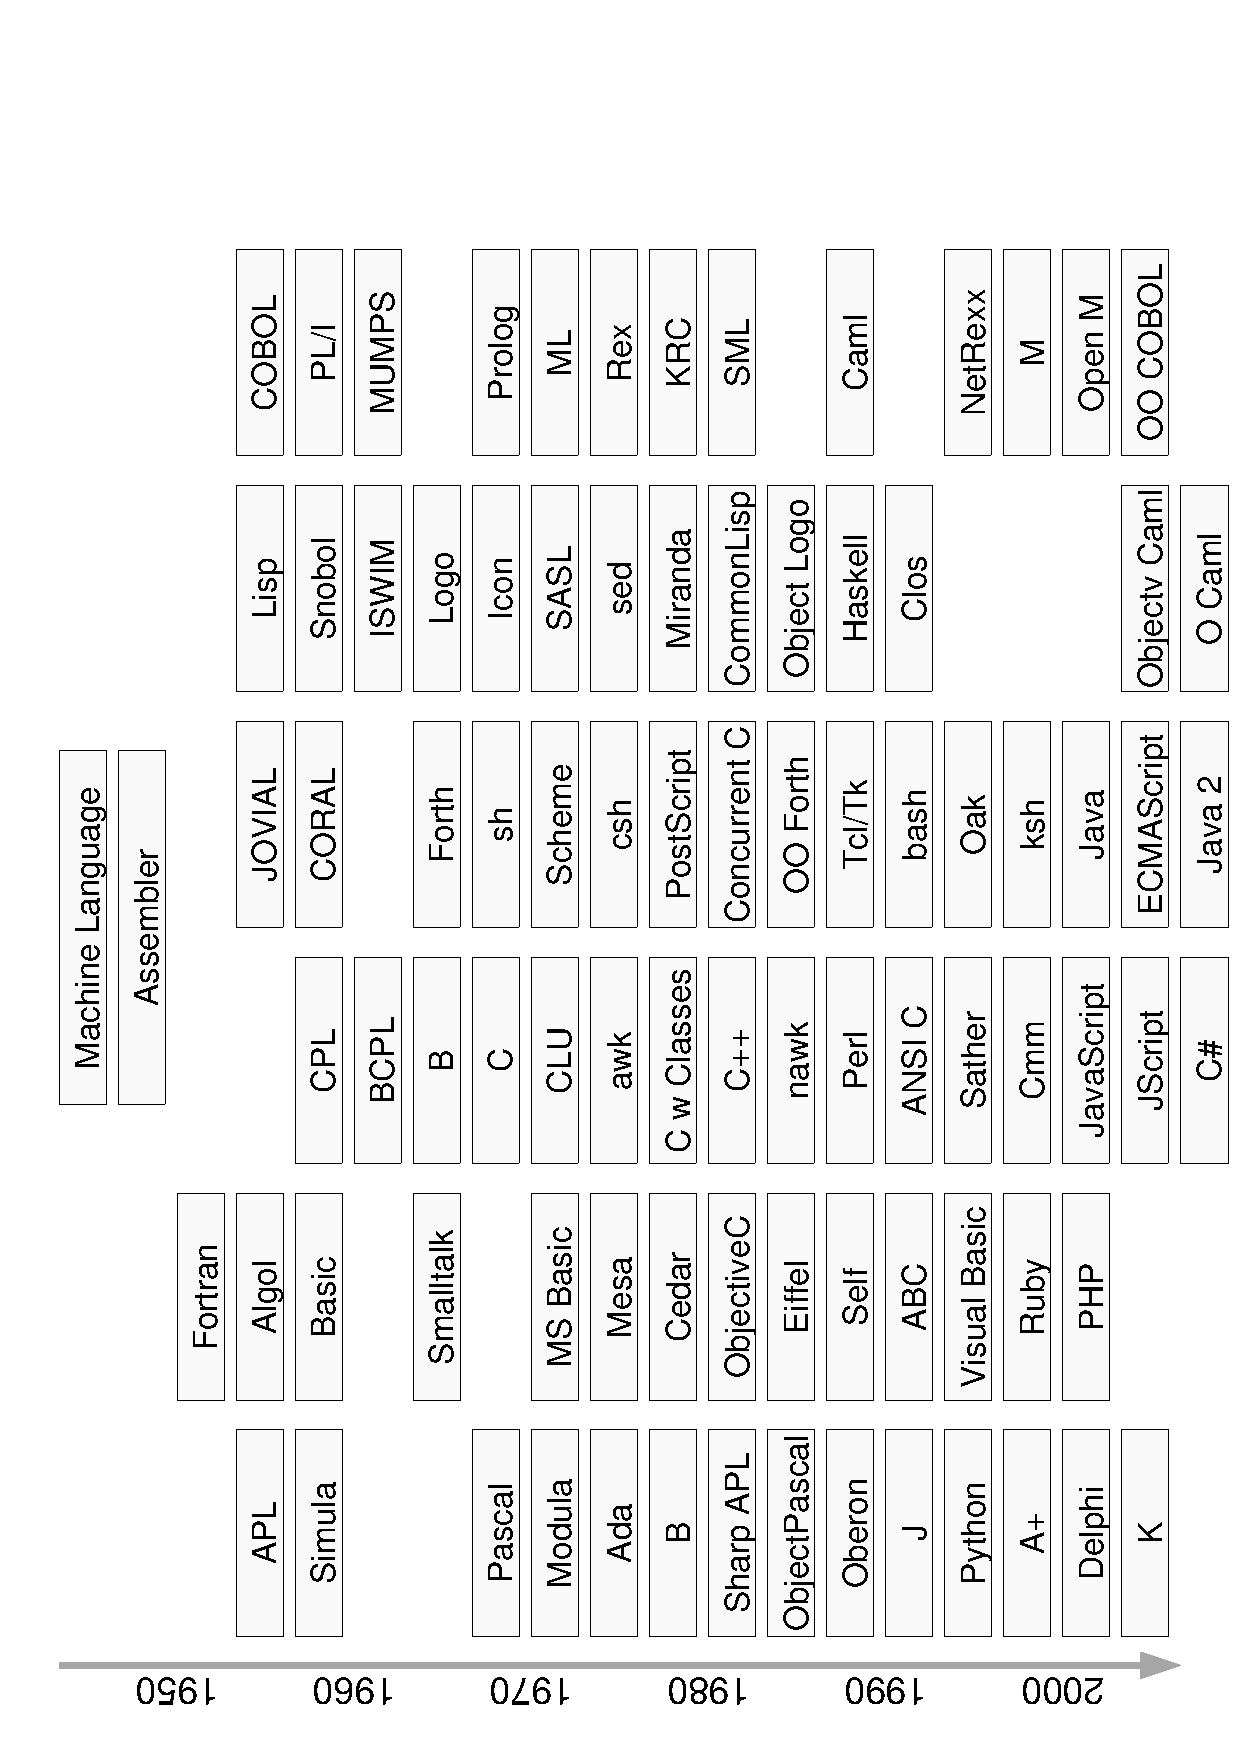
\includegraphics[scale=0.3,angle=-90]{graphic/language.pdf}
        \caption{Programming Language History}
        \label{language_figure}
    \end{center}
\end{figure}

A lineage can be identified for every language, some popular of which are shown
in the following list, the corresponding language name mentioned at first,
being followed by the names of the language's ancestors. The right-most
language represents the oldest ancestor. Only \emph{one} lineage of arbitrary
choice is considered for each language; most languages have \emph{further}
ancestors that are not mentioned here:

\begin{itemize}
    \item[-] \emph{Java 2:} Java 1, Oak, Cedar, Mesa, Algol, IAL, Fortran
    \item[-] \emph{C\#:} C++, C with Classes, C, B, BCPL, CPL, Algol
    \item[-] \emph{VB.NET:} Visual Basic, MS Basic, Basic, Algol
    \item[-] \emph{Delphi:} Object Pascal, Pascal, Algol
    \item[-] \emph{Oberon:} Modula, Pascal
    \item[-] \emph{Self:} Smalltalk, Simula, Algol
    \item[-] \emph{Tcl/Tk:} Tcl
    \item[-] \emph{Python:} ABC, B
    \item[-] \emph{Perl:} nawk, awk, Icon, Snobol
    \item[-] \emph{PHP:} PHP/FI, Perl
    \item[-] \emph{Ruby:} CLU, Pascal
    \item[-] \emph{Haskell:} Miranda, KRC, SASL, ISWIM
    \item[-] \emph{O Caml:} Objective Caml, Caml, SML, ML
    \item[-] \emph{OO COBOL:} COBOL, Flow-Matic, B-O
    \item[-] \emph{NetRexx:} Object Rexx, Rexx, Rex, PL/1 ANS, PL/M, PL/I, COBOL
    \item[-] \emph{Open M:} M, MUMPS
    \item[-] \emph{Scheme:} Common Lisp, Lisp
    \item[-] \emph{PostScript:} OO Forth, Forth
\end{itemize}

Other historical approaches assign each programming language to a special
\emph{Generation}. Commonly used programming language generations and some of
their representatives are shown following \cite{wikipedia}:

\begin{itemize}
    \item[-] \emph{First Generation Language}: machine-level language
    \item[-] \emph{Second Generation Language}: assembly language
    \item[-] \emph{Third Generation Language} (3GL): Fortran, Algol, COBOL, Basic, C, C++
    \item[-] \emph{Fourth Generation Language} (4GL): SQL, Mathematica, SAS, VB, MATLAB
    \item[-] \emph{Fifth Generation Language}: Prolog, OPS5, Mercury
\end{itemize}
